\section{Experimental Setup}
\label{sec:experiments}

\subsection{Dataset}
We use the \textbf{Sherwood Simulation Suite}~\cite{bolton2017sherwood} 60 Mpc/h Planck-cosmology volume at $2048^3$ resolution; the dev redshift is $z = 0.3$. Each snapshot ships 16{,}384 sightlines along a single axis at 2048 velocity bins per ray, with ground-truth $\tau_{HI}(v)$ stored as \texttt{tauH1\_2048\_n16384\_z0.300.dat}. Sherwood ships four feedback variants: $P_1$ (no feedback), $P_2$ (stellar wind), $P_3$ (wind $+$ AGN), $P_4$ (wind $+$ strong AGN), an ablation matrix over baryonic feedback prescriptions. We train one independent field per variant so a downstream feedback-classification probe cannot leak the label through a conditioning input. We report Tiers 1--3 across all four variants; the densest tier (Tier 4, $n_{\text{rays}}=16{,}384$) is not run --- the close-out characterization rests on the $n_{\text{rays}}=1024$ grid probe (\S\ref{sec:experiments:gridprobe}) and the project is not extended past it (\S\ref{sec:nextsteps:scope}).

\subsection{Evaluation Metrics}
Three primary structure gates are computed against the simulation ground truth on the rendered $F=e^{-\tau}$:
\begin{itemize}
    \item \textbf{1D flux power spectrum} $P_F(k_\parallel)$ (Hann-windowed periodogram, $dv/\sum w^2$ leakage compensation): $|\Delta P_F / P_F| < \GatePF$ averaged over $k_\parallel \in [10^{\PFkLoExp}, 10^{\PFkHiExp}]$ s/km~\cite{walther2018powerspectrum, boera2019thermal}.
    \item \textbf{Density-density cross-correlation} $\xi_{\hat\rho, \rho}(r)$ --- a Stark-style FFT cross-power, normalized by each field's global std and inverse-transformed, on the periodic 60 Mpc/h grid~\cite{lee2015, stark2015tomography}. The $\xi(r{=}2\,h^{-1}\,\text{Mpc}) > \GateXi$ bar is \emph{demoted} below: the estimator returns a cross-correlation \emph{function} that decays with $r$, not a per-lag coefficient, so even truth-vs-truth scores only $\XiCeiling$ at $r = 2\,h^{-1}$ Mpc and no field can reach $\GateXi$. We report $\xi$ ceiling-relative.
    \item \textbf{Flux PDF}: two-sample KS distance on $F$ restricted to $F \in [\PDFwinLo, \PDFwinHi]$ (cuts exclude saturated absorbers and continuum/metal-line residuals~\cite{lee2015}): KS $< \GateKS$.
\end{itemize}
The fiducial pass point is $P_1$, $z = 0.3$, $n_{\text{rays}} = 1024$. The integrator was re-validated end-to-end at production architecture; peak VRAM at the smallest tier is $\TonePeakVRAM$ GB, the anchor for the per-tier microbatch table of \S\ref{sec:method} (validation loop in suppl.).

\subsection{Stage 2b cost-survey: mean-flux anchor retraction}
\label{sec:experiments:cost-survey-sweep}
The Stage 2b cost-survey sweep ran the per-tier schedule across all four variants at Tiers 1--3 (12 banked cells, all PASS pre-registered safety rails; calibration and per-tier numerics in suppl.). Those runs used a broken anchor $\langle F\rangle_{\text{obs}} = 0.877$ --- a $z\!\sim\!2$ value mislabeled as $z=0.3$, retracted for the verified $\langle F\rangle_{\text{obs}}(z=0.3) = \AnchorMeanF \pm \AnchorMeanFsigma$~\cite{kirkman2007}. The structure gates ($P_F$, KS-PDF, $\xi_{\hat\rho,\rho}$) are anchor-invariant by construction (invariant to uniform rescaling of $\hat F$), so the calibration evidence survives the retraction; a separate corrected-anchor run (\texttt{pub-t1}, $50{,}000$ steps, four physics) supplies the structure-gate readout of \S\ref{sec:experiments:cosmological-eval}. The $\tau_{\max}=10$ cap is locked by a sensitivity sweep (suppl.).

\subsection{Production MLP: structure-gate readout}
\label{sec:experiments:headline}
Tab.~\ref{tab:headline-3gate} consolidates the structure-gate readout for the production MLP across the four Sherwood feedback variants at the corrected-anchor full publication schedule (\texttt{pub-t1}). Two of the three directly-evaluated gates fail. $P_F$ fails $4/4$ at $\PFfactorOverGateLo$--$\PFfactorOverGateHi\times$ the gate; the flux-PDF KS gate closes $3/4$ (bootstrap-robust; $P_2$ q84 $=\KSBootstrapQHiPtwo$ fails). Mean-flux closes $4/4$ at the seed=42 single-seed anchor, but the 5-seed sightline-level bootstrap CI overlaps the Kirkman+2007 anchor $[\AnchorMeanFLo, \AnchorMeanFHi]$ in only $2/4$ cells ($P_3$, $P_4$ marginal at q84). Training is single-seed (seed $=0$); KS and $\langle F_{\rm pred}\rangle$ carry 5-seed sightline-level bootstrap CIs ($K=\BootstrapK$ resamples per cell, prediction and truth-side seeds from independent PCG64 streams; anti-degeneracy audit PASS, suppl.), and $P_F$ is the seed=42 anchor.

\textbf{Honest gap: the 3D $\xi$ gate was never evaluated on the MLP.} The third gate, the 3D density cross-correlation, is a 3D estimator. The MLP is supervised on 1D flux and produces no 3D density cube, so it has no $\xi$-of-record in the gate's defined form; the value shown in Tab.~\ref{tab:headline-3gate} is a 1D-along-ray density-correlation surrogate, measured on the cost-survey $P_1$ checkpoint and anchor-invariant by construction. The surrogate decouples from the 3D estimator under scale-dependent degradation, so we do not read it as the gate. The MLP therefore \emph{fails two of three directly-evaluated gates}; the third was never evaluated on the MLP. The 3D structure result the project can report comes from the explicit-grid probe of \S\ref{sec:experiments:gridprobe}, which produces a 3D cube.

\textbf{Bootstrap-vs-seed=42 mean-flux divergence (symmetric-honesty disclosure).} The 5-seed bootstrap mean for $\langle F_{\rm pred}\rangle$ lies systematically below the seed=42 anchor by $\meanFseedDeviationRangeLo$--$\meanFseedDeviationRangeHi\sigma$ across all four cells (KS is not similarly biased; per-cell $\sigma$ in suppl.); we disclose this because the bootstrap softens rather than strengthens the single-seed reading, as our pre-registered honest-reporting protocol requires.

\begin{table*}[t]
    \centering
    \renewcommand{\arraystretch}{1.05}
    \setlength{\tabcolsep}{3.5pt}
    \footnotesize
    \begin{tabular}{l|cc|cc|cc|c}
    Cell & $\langle F_{\text{pred}}\rangle$ (mean $\pm \sigma$) & MF call & KS ($<\!\GateKS$, mean $\pm \sigma$) & KS call & $|\Delta P_F/P_F|$ ($<\!\GatePFdec$) & $P_F$ call & $r_\rho^{\log}$ ($>\!\GateXi$)$^\dagger$ \\
    \hline
    $P_1$ (no fdbk)     & $\meanFBootstrapMeanPone \pm \meanFBootstrapStdPone$ & \textbf{FAIL} (CI $<$ anchor) & $\KSBootstrapMeanPone \pm \KSBootstrapStdPone$ & \textbf{PASS} & $\mathbf{\PFresidPone}$ & \textbf{FAIL $\PFfactorOverGateHi\times$} & $\rrhoLogProxyPone$ (FAIL) \\
    $P_2$ (wind)        & $\meanFBootstrapMeanPtwo \pm \meanFBootstrapStdPtwo$ & \textbf{FAIL} (CI $<$ anchor) & $\KSBootstrapMeanPtwo \pm \KSBootstrapStdPtwo$ & \textbf{FAIL $1.5\times$} & $\mathbf{\PFresidPtwo}$ & \textbf{FAIL $3.8\times$} & --- (owed) \\
    $P_3$ (wind+AGN)    & $\meanFBootstrapMeanPthree \pm \meanFBootstrapStdPthree$ & \textbf{PASS} (q84 marginal) & $\KSBootstrapMeanPthree \pm \KSBootstrapStdPthree$ & \textbf{PASS} & $\mathbf{\PFresidPthree}$ & \textbf{FAIL $\PFfactorOverGateLo\times$} & --- (owed) \\
    $P_4$ (strong AGN)  & $\meanFBootstrapMeanPfour \pm \meanFBootstrapStdPfour$ & \textbf{PASS} (q84 marginal) & $\KSBootstrapMeanPfour \pm \KSBootstrapStdPfour$ & \textbf{PASS} & $\mathbf{\PFresidPfour}$ & \textbf{FAIL $\PFfactorOverGateLo\times$} & --- (owed) \\
    \hline
    Tally (bootstrap)   & \multicolumn{2}{c|}{\textbf{2/4 overlap anchor}} & \multicolumn{2}{c|}{\textbf{3/4 PASS}} & \multicolumn{2}{c|}{\textbf{0/4 PASS}} & 0/1 measured \\
    \end{tabular}
    \caption{\textbf{Main structure-gate readout: 4 Sherwood feedback variants ($P_1$--$P_4$) $\times$ 3 primary gates.} Configuration: \texttt{pub-t1}, $50{,}000$ steps, $n_{\text{rays}}=64$, seed $=0$, $\langle F\rangle_{\text{obs}}=\AnchorMeanF$~\cite{kirkman2007}. KS and $\langle F_{\rm pred}\rangle$ are reported with 5-seed sightline-level bootstrap ($K=\BootstrapK$ resamples, prediction and truth-side seeds from independent PCG64 streams; anti-degeneracy F1/F2 audit PASS, suppl.); $P_F$ residual reported at the seed=42 single-seed anchor. \textbf{Verdict: mean-flux 2/4 CIs overlap the Kirkman+2007 anchor at q84 ($P_3$/$P_4$ marginal); KS 3/4 PASS bootstrap-robustly ($P_2$ q84 $=\KSBootstrapQHiPtwo$ fails $1.5\times$); $P_F$ 0/4 PASS, uniformly $\PFfactorOverGateLo\times$--$\PFfactorOverGateHi\times$ over the $\GatePF$ bar.} $^\dagger$The 1D-along-ray density-correlation proxy $r_\rho^{\log}$ is a \emph{necessary-but-not-sufficient surrogate} for the full 3D $\xi_{\hat\rho,\rho}(r=2\,h^{-1}\,\text{Mpc})>\GateXi$ gate; the value shown is the cost-survey T3 checkpoint at $P_1$ (anchor-invariant); \texttt{pub-t1} re-evaluation owed and sequenced behind \S\ref{sec:nextsteps}.}
    \label{tab:headline-3gate}
\end{table*}

\subsection{\texorpdfstring{Cosmological evaluation: $P_F$ falsifies the rescale-preview reading}{Cosmological evaluation: PF falsifies the rescale-preview reading}}
\label{sec:experiments:cosmological-eval}
The cost-survey ``rescale-as-preview'' reading is falsified by the trained-at-target result: $4\times$ more training and the corrected anchor \emph{increased} $|\Delta P_F/P_F|$ at $P_1$ (overlay in suppl.). At the corrected anchor and full schedule (per-cell values in suppl.), the four-physics \texttt{pub-t1} bundle closes mean-flux $4/4$ (cross-physics spread $\meanFseedFortyTwoSpread$, $<\!1\%$) and the flux-PDF KS gate $3/4$, while $|\Delta P_F/P_F|$ stays uniformly $\PFfactorOverGateLo\times$--$\PFfactorOverGateHi\times$ over the $\GatePFdec$ gate. Matched mean-flux and near-uniform KS closure with a uniformly $\sim\!4\times$-over $P_F$ residual is inconsistent with a calibration deficit: \emph{$P_F$ is structurally bound, not calibration-bound}. The gap is in second-order spectroscopic statistics that survive matched mean-flux and matched flux PDF, and it is not an MLP-capacity limit --- the explicit-grid probe (\S\ref{sec:experiments:gridprobe}) shows it persists at the maximal-capacity parameterization. Log-space $\tau$-MSE is not a sufficient proxy for the structure gates (suppl.).

\subsection{\texorpdfstring{$\tau$-binned residual decomposition: saturation-regime under-fitting, positively identified cross-physics}{tau-binned residual decomposition: saturation-regime under-fitting, positively identified cross-physics}}
\label{sec:experiments:tau-binned}
The structural-$P_F$ verdict states \emph{that} the gap is in second-order spectroscopic statistics; a $\tau$-binned residual decomposition over the four \texttt{pub-t1} checkpoints (seven $F$-bins matching the saturated-absorber partition of \S\ref{sec:method:loss}) locates \emph{where} it lives. The saturation-band concentration ratio $R = (\text{residual-mass share})/(\text{pixel-mass share})$ exceeds the positive-ID floor $R \geq \GateRsatFloor$ by $>\!\RsatFactorOverFloor\times$ in all four cells (range $\RsatRangeLo$--$\RsatRangeHi$, $\sim\!\RsatSpreadRelative$ cross-physics spread; per-cell $R$ and 4-panel residual-mass histograms in suppl.), while the linear regime contributes only $|\langle\Delta F\rangle| \leq \RsatLinearBandResidual$; the in-band Pearson $r_{\text{pearson}}(\tau) = \RsatPearsonTauPone$ at $P_1$ shows the $\tau$-rank order collapses where it matters most for $P_F$, ruling out a global $\tau$ rescaling. The decomposition positively identifies the saturation regime as the residually-supported mechanism cross-physics; it does not claim the gap's cause, which the explicit-grid probe (\S\ref{sec:experiments:gridprobe}) then localizes to the under-constraint of the inverse problem.

\subsection{Explicit-grid probe: the flux inverse problem is under-constrained}
\label{sec:experiments:gridprobe}
The MLP diagnosis of \S\ref{sec:experiments:cosmological-eval}--\S\ref{sec:experiments:tau-binned} localizes the residual but leaves one question open: is the saturation-band deficit a capacity limit of the implicit field, or a property of the inverse problem? We answer with the explicit-voxel-grid probe of \S\ref{sec:method:gridprobe} --- four free-per-voxel grids at $\GridG^3$, plain flux supervision, one lever, at $P_1$, $z = 0.3$, $n_{\text{rays}} = 1024$ ($50{,}000$ steps).

\textbf{Trainability: the grid escapes the optimization collapse.} The grid's predicted-flux-power-band variance is $\VarPfBandRatio$, flat from step $5{,}000$ to $50{,}000$ --- about $1000\times$ over the collapse bar that retired the interventions of \S\ref{sec:nextsteps:pf}. The grid trains. Its variance sits at the same $\approx\!1.0$ level as the healthy MLP run, so it lands in the same saturation-band partial-underfit basin (Mode A) at the most-expressive parameterization; this is the representation-invariance of that basin landing, scoped to $P_F$.

\textbf{Decisive evidence (K2): the grid beats the truth on flux.} We forward-model the \emph{true} sightline fields ($\rho, T, X_{HI}, v_{\text{pec}}$ at the ray points) through the same integrator under the same log-space loss --- RSD applied identically, amplitude $\tau_{\text{amp}}$ free --- and minimize over $\tau_{\text{amp}}$. The true field scores data loss $\KTwoTruthLoss$; the grid scores $\KTwoGridLoss$, about $\KTwoMarginFactor\times$ better. The grid fits the observed flux better than the true field does through the same forward model. The margin is amplitude-flat (the true-field loss is flat over $\tau_{\text{amp}} \in [0.2, 4]$), which rules out the amplitude-calibration escape; the non-trivial content is the $\KTwoMarginFactor\times$ margin and that flatness, not the bare $\text{grid} < \text{truth}$ inequality. The margin includes integrator-induced slack: the $\KTwoTruthLoss$ floor is our FGPA-vs-radiative-transfer integrator error, not a physical residual, and the grid can exploit slack the truth cannot. The reading is that the flux through this forward model does not identify the true 3D field --- the $z = 0.3$ flux inverse problem is under-constrained. We do not separate problem-intrinsic from forward-model-induced under-determination at $\langle F\rangle = \MeanFluxZpThree$ (Fig.~\ref{fig:k2-degeneracy}).

\begin{figure}[t]
    \centering
    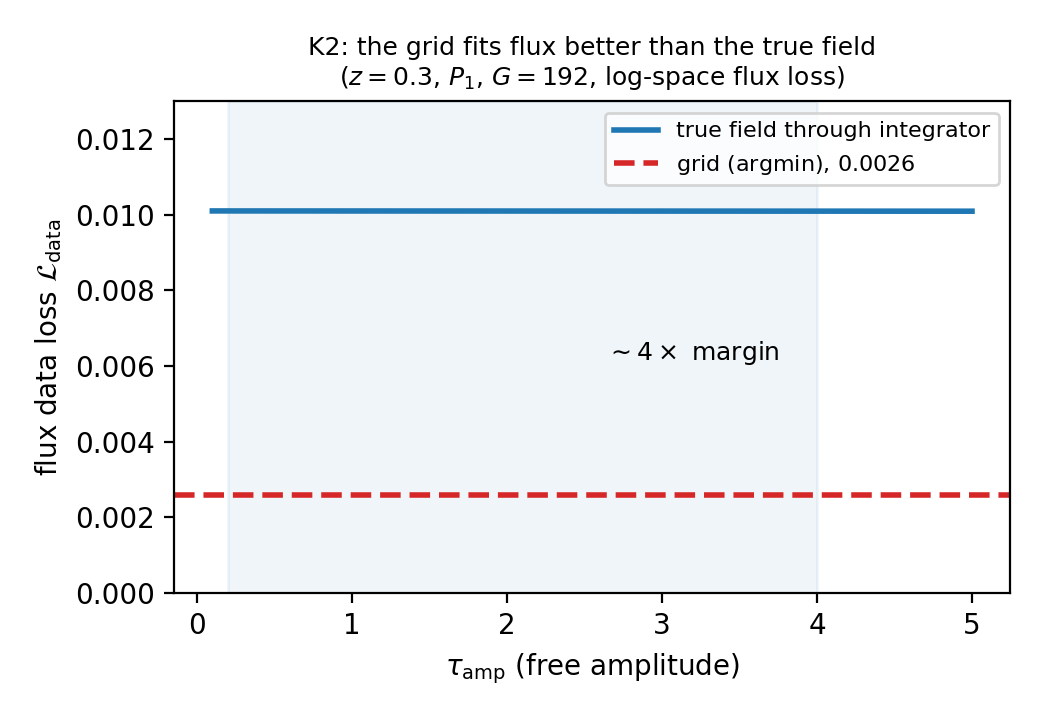
\includegraphics[width=0.84\linewidth]{figures/d73_k2_truth_vs_grid.png}
    \caption{\textbf{K2 degeneracy ($z{=}0.3$, $P_1$, $G{=}192$, log-space flux loss).} The true sightline fields forward-modeled through the same integrator (free $\tau_{\text{amp}}$) score flux data loss $\KTwoTruthLoss$, flat over $\tau_{\text{amp}}\in[0.2,4]$ (shaded); the trained grid scores $\KTwoGridLoss$ (dashed), about $\KTwoMarginFactor\times$ lower. \emph{Verdict:} the grid fits the flux better than the true field does, so the flux optimum does not identify the true 3D field --- the inverse problem is under-constrained under this forward model. The amplitude-flatness rules out a calibration escape.}
    \label{fig:k2-degeneracy}
\end{figure}

\textbf{The grid closes the flux-power gate the MLP failed.} Measured directly on the trained grid (same \texttt{compute\_p\_flux} convention as the gate), the grid's $|\Delta P_F/P_F|$ band-mean over $k_\parallel \in [10^{-2.5}, 10^{-1.5}]$ s/km is $\PFresidGrid$ --- a \emph{PASS} of the $10\%$ gate, against the production MLP's $\PFresidGridBaseline$ FAIL.\footnote{The MLP baseline is the $n_{\text{rays}}=64$ \texttt{pub-t1} anchor and the grid is $n_{\text{rays}}=1024$; same estimator convention and the same $10\%$ gate, so the PASS/FAIL verdicts are directly comparable, but the residual magnitudes are not a controlled same-config contrast.} So the explicit field does close the scalar flux-power statistic the implicit MLP could not --- yet, as the cross-correlation below shows, it does not recover the 3D field. This is the sharp form of the under-constraint: the grid passes \emph{both} flux gates (band variance and power spectrum) and beats truth on flux loss, while the 3D structure stays wrong.

\textbf{Supporting evidence: weak 3D structure, ceiling-relative.} The grid's 3D density cross-correlation at $r = 2\,h^{-1}$ Mpc is $\XiGrid$. The $\GateXi$ acceptance bar is demoted on two grounds, both confirmed first-hand. First, the estimator returns a cross-correlation function that decays with $r$: truth-vs-truth scores $\XiCeiling$ at $r = 2\,h^{-1}$ Mpc, not $\approx\!1.0$, so no field can pass $\GateXi$ and the ``$\XiGrid$ vs.\ $\GateXi$'' reading is invalid. Read ceiling-relative, the grid recovers $\XiCeilingFraction$ of the field's own achievable $r = 2\,h^{-1}$ Mpc autocorrelation and sits below truth-plus-100\%-noise ($\XiTruthNoiseHundred$) --- weak structure recovery. Second, a real-space-cube-vs-redshift-space-flux frame mismatch confounds $\xi(r = 2)$: the estimator scores a real-space cube against real-space truth while supervision is redshift-space flux with no RSD remap, and at $z = 0.3$ the displacement is $\Delta\chi_{\text{rms}} = \FrameDeltaChiRms$, $\Delta\chi_{\text{p95}} = \FrameDeltaChiPNF\,h^{-1}$ Mpc, comparable to the $r = 2\,h^{-1}$ Mpc gate scale. The mismatch depresses $\xi(r = 2)$ independent of reconstruction quality, on both this neural number and the idealized Wiener baseline (lower bound $\WienerXiLowerBound$, optimum un-pinned). $\xi$ is therefore supporting, not load-bearing; K2 carries the close. A corrected per-lag coefficient is banked as future work (\S\ref{sec:nextsteps}). Fig.~\ref{fig:xi-ceiling} shows the $\xi(r)$ profiles ceiling-relative.

\begin{figure}[t]
    \centering
    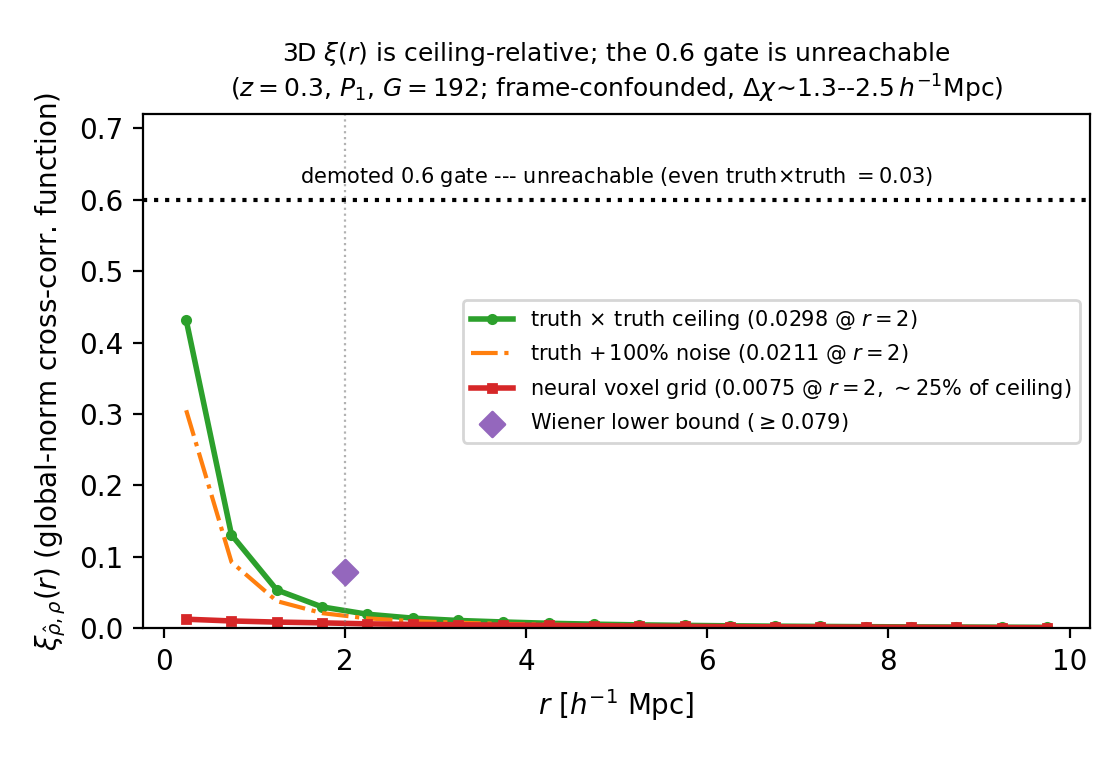
\includegraphics[width=0.84\linewidth]{figures/d73_xi_ceiling_relative.png}
    \caption{\textbf{3D $\xi(r)$ is ceiling-relative; the $\GateXi$ gate is unreachable ($z{=}0.3$, $P_1$, $G{=}192$).} Even truth-vs-truth reaches only $\XiCeiling$ at $r{=}2\,h^{-1}$Mpc under the implemented global-normalized estimator, so the dotted $\GateXi$ bar cannot be passed by any field. The neural grid ($\XiGrid$) recovers $\XiCeilingFraction$ of that ceiling and sits below truth-plus-100\%-noise ($\XiTruthNoiseHundred$); the Wiener lower bound ($\geq\!\WienerXiLowerBound$) is shown for context. \emph{Verdict:} weak structure recovery, not a $\GateXi$-gate ``catastrophic fail''; the comparison is additionally frame-confounded ($\Delta\chi\!\sim\!\FrameDeltaChiRms$--$\FrameDeltaChiPNF\,h^{-1}$Mpc at the gate scale).}
    \label{fig:xi-ceiling}
\end{figure}

\textbf{Reading.} At $z = 0.3$ ($P_1$), a maximal-capacity-within-this-study free-per-voxel field ($\GridG^3$), trained under the production flux supervision, closes the flux-power gate the production MLP failed ($|\Delta P_F/P_F| = \PFresidGrid$ vs.\ $\PFresidGridBaseline$, PASS vs.\ FAIL) and fits the observed flux about $\KTwoMarginFactor\times$ better than the true field does through the same forward model ($\KTwoGridLoss$ vs.\ $\KTwoTruthLoss$), yet recovers only weak 3D structure. Escaping the optimization collapse is necessary but not sufficient: the flux through this integrator --- even when it passes the community flux-power gate --- does not determine the 3D field. We make no claim beyond $z = 0.3$.

\subsection{Substrate-discriminability probe at the reconstruction scale}
\label{sec:experiments:substrate-probe}
A separate question is what cross-physics signal the truth density field carries at the spatial scale a downstream 3D consumer would slice it on. We answer with a probe-classifier construction~\cite{alain_bengio2017probing}: a 3D ResNet-18 ($\SubstrateProbeParams$ parameters) is trained to assign $\SubstrateProbeCropSize^3$-voxel crops of the truth $\rho/\bar\rho$ field ($\SubstrateProbeBoxMpc\,h^{-1}$ Mpc on a side, matched to the $\xi_{\hat\rho,\rho}$ evaluation scale) to one of the four Sherwood feedback variants, against a pre-registered two-scalar $[\text{mean}, \text{variance}]$ anti-degeneracy floor~\cite{geirhos2020shortcut}. The 3D ResNet reaches $\hat A_{\text{overall}} = \SubstrateProbeAcc$ against the $\SubstrateProbeMeanVarAcc$ moment-only baseline (chance $\SubstrateProbeChance$); the $\SubstrateProbeMarginPP$ pp margin is below the pre-registered $\SubstrateProbeADfiveBarPP$ pp floor, so we decline to publish $\hat A_{\text{overall}}$ as a substrate accuracy number. Cross-physics separability of the Sherwood variants is established elsewhere at the 1D Ly$\alpha$ flux-statistic scale~\cite{bolton2017sherwood, irsic2017xq100}; at this $\SubstrateProbeCropSize^3$ density-crop substrate the 3D ResNet does not surface signal beyond two summary moments. Bootstrap CIs, the per-quintile curve, and the confusion-matrix structure are in the supplementary.

\subsection{Open evaluation axes and compute footprint}
\label{sec:experiments:compute}
Validation, Tiers 1--3 across four variants, and the four-cell \texttt{pub-t1} bundle consumed approximately \GPUHoursSpent\ GPU-hours. Two evaluation axes are banked as future work, not opened here (\S\ref{sec:nextsteps:scope}): (a) re-evaluating the 1D-along-ray density correlation $r_\rho^{\log}$ on the corrected-anchor checkpoints --- the cost-survey value $\rrhoLogProxyPone$ at $P_1$ is anchor-invariant by construction and carries unchanged; and (b) the corrected per-lag 3D $\xi_{\hat\rho,\rho}(r=2\,h^{-1}\,\text{Mpc})$ coefficient, which needs the grid cube and remains frame-mismatch-confounded (\S\ref{sec:experiments:gridprobe}).
